\documentclass[tikz,border=5pt]{standalone}
\usepackage{tikz}
\usepackage{pgfplots}
\pgfplotsset{compat=1.18}

\begin{document}
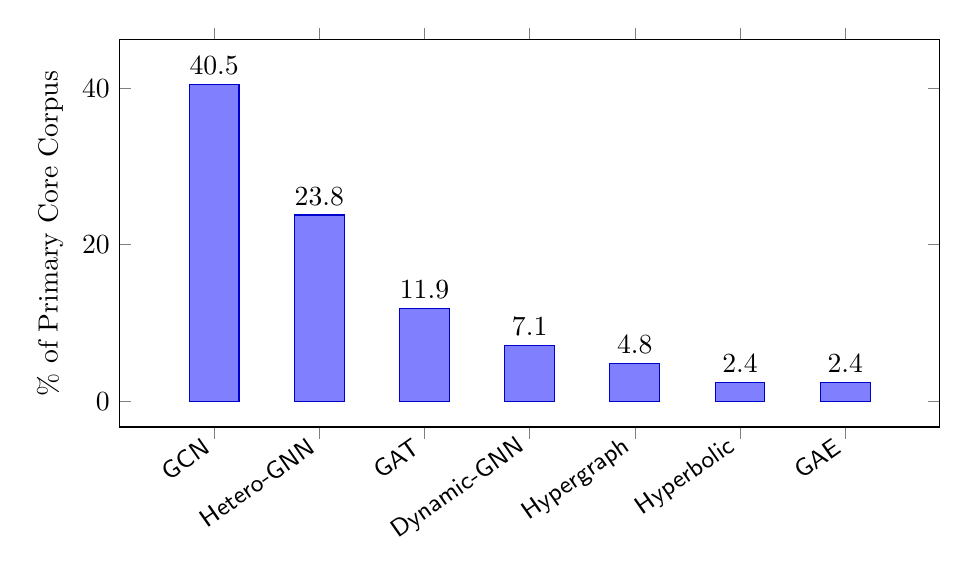
\begin{tikzpicture}
\begin{axis}[
    ybar,
    enlargelimits=0.15,
    legend style={at={(0.5,-0.25)}, anchor=north,legend columns=-1},
    ylabel={\% of Primary Core Corpus},
    symbolic x coords={GCN, Hetero-GNN, GAT, Dynamic-GNN, Hypergraph, Hyperbolic, GAE},
    xtick=data,
    x tick label style={rotate=35,anchor=east,font=\sffamily\small},
    nodes near coords,
    nodes near coords align={vertical},
    width=12cm,
    height=6.5cm,
    bar width=18pt,
    fill=blue!60!black
]
\addplot[fill=blue!50!white, draw=blue!80!black] coordinates {
    (GCN,40.5) 
    (Hetero-GNN,23.8) 
    (GAT,11.9) 
    (Dynamic-GNN,7.1) 
    (Hypergraph,4.8) 
    (Hyperbolic,2.4) 
    (GAE,2.4)
};
\end{axis}
\end{tikzpicture}
\end{document}
